

% \TODO{Cite the XA distributed transaction model}.
% \TODO{Cite Corda Tearoffs}.
% \TODO{Cite Fabric private transactions} mentioned in DAML blog post.
% https://medium.com/daml-driven/keeping-smart-contracts-private-is-hard-unless-you-truly-understand-them-920b31d723e4

% TODO: How does a confirming party know which other parties to ask for confirmations?
% It may see some in the facts revealed to it, but if a fact has been blinded it may not
% know it can ask the parties listed in that fact. We may want to add an extra field
% to the transaction listing the parties involved, which is separate from the facts
% themselves. This seems like a design variable where we might want the extra list,
% or not, and both answers are valid.


% -----------------------------------------------------------------------------
\section{Privacy}
\label{s:Privacy}

\begin{figure}
\begin{center}
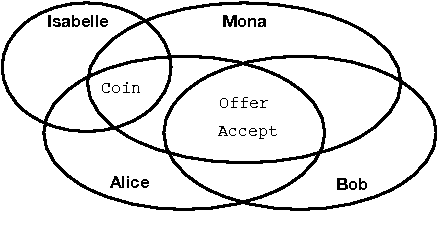
\includegraphics{figure/coin-transfer-visibility.pdf}
\end{center}
\vspace{-2ex}
\caption{Fact Visibility for Monitored Coin Transfer}
\label{f:CoinTransferVisibility}
\end{figure}

In practical multi-party workflows it is often not desirable, or not legal, for all data used in the workflow to be provided to all parties. In the coin transfer example from \S\ref{s:FactsWeights}, we could assume that Alice would not want to reveal the total number of coins she holds to Bob, nor the item she wishes to purchase (the Guitar) to Isabelle. Conversely, it is often the case that the details of workflows \emph{must} be revealed to third parties that do not themselves authorize any of the facts used in the workflow. Details of transactions may be required to be sent to financial regulators that monitor the operation of markets, or to credit agencies that offer loans based on the spending patterns of their clients. For the sake of example, we extend the coin transfer workflow described in the previous section with an extra party, Mona, who monitors all coin transactions. Figure~\ref{f:CoinTransferVisibility} shows who can see which facts in diagramatic form. The associated transfer rule is as per Figure~\ref{f:CoinTransfer}, extending by listing Mona listed as an observer of the produced coin fact.

% TODO: refer back to the store data model to say each party has their own fragment of the state.


% -----------------------------------------------------------------------------
\subsection{Transaction and Validation}
\label{s:Transactions}
Assume that Alice, Bob, Mona and Isabelle have their own computers in their own offices, each containing a subset of facts as per Figure~\ref{f:CoinTransferVisibility}. Each party also has a copy of the extended transfer rule. Alice decides that it time to perform the transfer, and builds the following transaction structure:

\begin{small}
\begin{code}
Transaction
 seq    = ... sequence number ...
 rule   = ... hash of the transfer rule ...
 input  = [ Offer [id = '1234, terms = "To purchase a Guitar"
                  giver = !Alice, receiver = !Bob]
            by  {!Alice}            obs {!Mona, !Bob}
            use {'transfer}         num  1

          , Accept [id = '1234, accepter = !Bob]
            by  {!Bob}              obs {!Mona, !Alice}
            use {'transfer}         num 1

          , Coin   [issuer = !Isabelle, holder = !Alice]
            by  {!Isabelle, !Alice} obs {!Mona}
            use {'transfer}         num 1 ]

 output = [ Coin   [issuer = !Isabelle, holder = !Bob]
            by  {!Isabelle, !Bob}   obs {!Mona}
            use {'transfer}         num 1 ]
\end{code}
\end{small}

The transaction includes a fresh sequence number as an identifier, the hash of the code of the transfer rule, the list of facts being spent (input) by the transaction, and the list of new fact created (output). Alice would now like the other parties to agree that this is a valid execution of the transfer rule, and update their own local databases. However, as per Figure ~\ref{f:CoinTransferVisibility} not all parties are entitled to see all facts listed in the transaction.

Recall from \S\ref{s:Observation} that a party $P$ can see a fact $F$ when it is listed in either its \emph{by-authority} set or its \emph{obs-authority} set. We express this as a simple predicate, where the functions \trm{auth-by} and \trm{auth-obs} retrieve the respective annotations from a fact value.
$$
\trm{sees}~ P~ F = |(\trm{auth-by}~F \cup \trm{auth-obs}~F) \cap \{P\}| \ge 0
$$
Applying this predicate to the facts in the transaction, Alice computes that 1) the @Offer@ and @Accept@ should be visible to Alice, Bob and Mona; 2) the input @Coin@ fact should be visible to Isabelle, Alice and Mona, and 3) the output @Coin@ fact should be visible to Isabelle, Bob and Mona. Importantly, the details of the transaction do not reveal how many coins Alice might happen to have when she builds it. Isabelle and Mona will already know how many coins Alice, has as they have seen previous coin transactions, but there is no reason for this information to appear in the transaction structure itself.

Alice cannot send the complete transaction to all parties as they are not all entitled to see all the facts. Instead, Alice sends a \emph{restricted view} for each of the other parties using the `sees' predicate above, blinding the facts that a particular party is not entitled to see from their view.


% -----------------------------------------------------------------------------
\subsection{Transaction Views}
For the sake of presentation we will abbreviate the four weighted facts in the transaction from \S\ref{s:Transactions} as $d_1, d_2, d_3, d_4$. We use the letter $d$ as a mnemonic short for \emph{factoid} --- being an ``unreliable'' fact, because the weight might be zero. We express the complete transaction as the following tuple, using $h(X)$ to mean the hash of value $X$.
$$
 (seq,~ h(tx), [d_1, d_2, d_3], [d_4])
$$
The above tuple contains the transaction sequence number, the hash of the transaction rule code, the list of input factoids, and list of output factoids. The views for each party are computed by replacing some of the factoids by their \emph{blinded hashes}. A blinded hash is a cryptographic hash which has been combined with a random salt value, so that the source data cannot feasibly be recovered by brute force guessing. We write $s_1 .. s_4$ as the salts for each factoid.

Before computing the view for each party, Alice first computes an overall transaction identifier by replacing all factoids in the transaction with their blinded hashes, then hashing the result:
$$
\begin{array}{rl}
 \hspace{-2ex} h((seq,~ h(tx), [h(d_1, s_1), h(d_2, s_2), h(d_3, s_3)], [h(d_4, s_4)]))
\end{array}
$$
This is a unique(ish) identifier for the transaction, provided the hash values are long enough that there will not be collision in practice.

Now, as Isabelle is entitled to see the @Coin@ facts but not the @Offer@ or @Accept@ facts, she receives a view containing the fact data and salt values for the @Coin@ facts, but only the blinded hashes of the @Offer@ and @Accept@ facts:
$$
\trm{for Isabelle:}~~(seq,~ h(tx), [h(d_1, s_1), h(d_2, s_2), (d_3, s_3)], [(d_4, s_4)])
$$
Similarly, Bob is entitled to see the @Offer@, @Accept@ and produced @Coin@ fact, but not the consumed @Coin@ fact, so receives a corresponding view. In this particular example Bob will be able to use the definition of the @transfer@ rule to infer what the consumed coin fact must have been anyway, but we will discuss this in the next section.
$$
\trm{for Bob:}~~(seq,~ h(tx), [(d_1, s_1), (d_2, s_2), h(d_3, s_3)], [(d_4, s_4)])
$$
Finally, Mona is entitled to see all the facts, so she gets the full unblinded transaction.
$$
\trm{for Mona:}~~(seq,~ h(tx), [(d_1, s_1), (d_2, s_2), (d_3, s_3)], [(d_4, s_4)])
$$
All four parties, including Alice, will be able use their own view to compute the same transaction identifier. Isabelle was not given the data for the @Offer@ and @Accept@ facts, but as she knows their hashes she can still compute the hash of the overall transaction. Isabelle \emph{can} determine that the giver and receiver fields of the @Offer@ fact must have contained the values @!Alice@ and @!Bob@ respectively. Isabelle knows the rule that the transaction was generated from, and the rule says that the giver and receiver of an @Offer@ must match the corresponding fields of the input @Coin@ facts that she does see. However, Isabelle cannot see that the coin is being transferred @"To purchase a Guitar"@, because that information is was only present in the @Offer@.


% -----------------------------------------------------------------------------
\subsection{Consensus}
Once each party has received their own transaction view, they can compare it against their own fragment of the ledger state and confirm with each other whether their views are valid. The fragment of ledger state visible to Isabelle contains the total weight of @Coin@ facts currently held by Alice. When Bob confirms with Isabelle that her view of the transaction is valid, this tells Bob whether Alice actually has a coin to transfer to him. Similarly, when Isabelle confirms with Bob that his view of the transaction is valid, this tells Isabelle that Bob really did agree to the transfer. In a practical workflow Isabelle might represent a commercial Bank, and in this case Bob would likely trust Isabelle to answer truthfully when asked if enough coins are available for a transfer, even though he does not want her to know that he is adding to his collection of guitars.

There are many ways to manage the confirmation process in a concrete implementation. For a small number of parties, such as to manage commercial workflows between banks, it may be sufficient for each party to confirm the transaction directly with all others. This would require $O(n^2)$ confirmations in practice, but in the happy case the only information that needs to be exchanged is that the confirming party agrees with the transaction view identified by its hash code. For a greater number of parties, cryptographically signed confirmation messages could be propagated with a peer-to-peer protocol~\cite{El-Ansary2003:Broadcast}, or Byzantine Fault Tolerant (BFT) consensus protocol~\cite{Lamport1982:Byzantine, Ongaro2014:Consensus, Gilad2017:Algorand}.

Alternatively, @Mona@ could represent a monitoring company that simply receives transaction views and archives them. For applications where the parties know each other and are expected to be honest, there may not be a need to synchronously confirm each transaction. If there are any disputes between Alice, Bob or Isabelle, then they could retrieve the views given to Mona and validate that the transaction hashes of those views match their own.


% -----------------------------------------------------------------------------
\subsection{Nested Transactions}
\label{s:NestedTransactions}
For the transaction in \S\ref{s:Transactions}, Isabelle's view is constructed by blinding the @Offer@ and @Accept@ facts, as Isabelle is not an observer of these. Blinding these facts means that that Isabelle cannot use the input list to directly execute the rule and check the output. In a concrete application where there is a trusted monitor, such as Mona, this would not matter as the other parties would expect Mona to answer truthfully whether her transaction view is valid. If we instead wish to allow Isabelle to validate the output list in her own view, we can split the transfer rule into two parts: one that combines Alice's offer with Bob's agreement, and another to perform the actual coin transfer.

\begin{small}
\begin{code}
  rule  agreeOnOffer
  await Offer  [id = ?i, giver = ?g, receiver = ?r] gain {g}
    and Accept [id = ?i, accepter = ?r]             gain {r}
  to
    say Agreed [giver = g, receiver = r]
     by {g,r}  obs {!Mona,!Isabelle}

  rule  doTheTransfer
  await Agreed [giver = ?g, receiver = ?r]        gain {g,r}
   and  Coin   [issuer = !Isabelle, holder = g]
        gain {!Isabelle,g}
  to
    say Coin   [issuer = !Isabelle, holder = r]
     by {!Isabelle,r} obs {!Mona}
\end{code}
\end{small}

With these two rule definitions Alice can build a nested transaction \CITE, which is a list containing the subtransactions for each of the rule firings. For the above rules, the first sub-transaction will consume the @Offer@ and @Accept@ facts to produce an @Agreed@ fact that is authorized by both Alice and Bob. The second sub-transaction will then immediately consume this @Agreed@ fact along with the @Coin@ fact, to produce the new @Coin@ fact. Both the created @Agreed@ fact in the first transaction, as well as the input @Coin@ fact are guaranteed to be visible to Isabelle, so she will be able to re-run the second sub-transaction and validate the output herself. Isabelle will still not be able to see the terms of the offer, but will be able to confirm with Bob that he agreed to it.

In related work, the DAML~\cite{DA2019:DAML} ledger model is a more object oriented version of our own system. DAML combines facts and rules into a \emph{contract instance}, similar to an object in an OO model, where our facts are the object's fields, and our rules its methods. Parties using the system authorize whole objects, instead of using separate systems for the authorization of facts (our by-authority set) and rules (our use-set). The DAML model is based on UTxO~\cite{Zahnentferner2018:UTxO}, so invoking a method on an object typically causes it to allocate some new objects and consume (or ``spend'') the called object.

A design decision of DAML is to ensure that each party that authorized an object is able to re-execute the subtransaction that consumes their object. This can require the system to \emph{divulge} additional objects to an authorizing party that where not visible until the object they authorized is consumed. However, the object oriented code structure of DAML causes the transactions produced by method invocation to have a nested form similar to the above. In DAML, the details of the equivalent @doTheTransfer@ subtransaction can be sent to @Isabelle@, leaving the details of @agreeOnOffer@ private between Alice and Bob.

% TOOD: in transfer, auth of 'g' is gained but not used. This is added to check the agreement is really authorized by 'g'. Can probably work this into the auction example.


% -----------------------------------------------------------------------------
\subsection{Incidental Observers}
In the transaction structure from \S\ref{s:Transactions} note that although Alice is the one forming the transaction, she herself is not listed as an observer of the output @Coin@ fact. When Alice computes the restricted views for Bob, Isabelle and Mona she knows that those parties will add this output fact to their own stores, but she should not add it to her own. As Alice is not an observer for this fact, any other party that builds a transaction that consumes this fact will not inform her that this has happened. In this case we say that Alice is an \emph{incidental observer} of the output @Coin@ fact.

% In a related point, although Bob is not listed as an observer of the input @Coin@ fact, the transaction view that he receives includes enough information for him to determine most of its contents. According to the rule definition the fields of the input coin fact must match other fields in the input @Accept@ and output @Coin@ facts that he can see. However, in general, Bob will not know the obs-authority set of the input @Coin@, as this is not fixed by the rule.


% -----------------------------------------------------------------------------
\subsection{Upgrade}
\label{s:Upgrade}
In practical systems it is often necessary to upgrade data formats and business rules as requirements change over time. As the use-sets attached to each fact are sets of rule names that can be manipulated from the term language, it is easy to construct rules that perform upgrades.

\begin{small}
\begin{code}
  rule  upgrade
  await Coin [issuer = ?s, holder = ?h]   gain {s, h}
    and LetsUpgrade [party = s, rules = ?rs] gain {s}
    and LetsUpgrade [party = h, rules = ?rs] gain {h}
   to
    say Coin [issuer = s, holder = h]
     by {s, h} use rs
\end{code}
\end{small}

Provided the upgrade rule is listed in the use-set of the original @Coin@, this rule allows the issuer and holder to upgrade it to another one, possibly listing different rules. There is no need for a privileged operator party to orchestrate the upgrade. The meaning of facts is controlled by the parties that authorize them, not the people  that run the ledger system, which we will return to in \REF.


% -----------------------------------------------------------------------------
\begin{figure}
\begin{center}
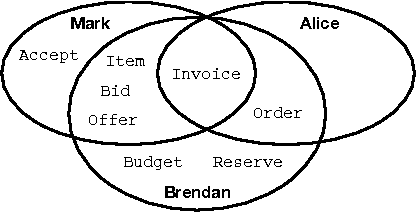
\includegraphics{figure/auction-visibility.pdf}
\end{center}
\vspace{-2ex}
\caption{Fact Visibility in Auction Example}
\label{f:AuctionVisibility}
\end{figure}


\subsection{Query}
\label{s:Query}
In the examples we have presented so far, each matching clause in a rule has always selected a single fact at a time. In contrast, consider an auction workflow where we will need to rank offers by price, instead of just selecting any which matches. The fact visibility of such a workflow is depicted in Figure~\ref{f:AuctionVisibility}. Mark runs the auction market, Brendan is a broker, and Alice is a customer. The house rules are such that a customer (Alice) may not bid on items directly. Instead, the customer enlists a broker (Brendan) to which they provide an @Order@ describing the sort of @Item@ they wish to purchase, and their price limit. Naturally, the details of the @Order@ are private between the broker and customer, as the party running the auction house should not know the absolute maximum price a customer is willing to pay. During the auction, the market announces which items are for sale, including their lot number, description, and asking price. If anyone wishes to pay the asking price then the item is sold immediately. Bids may also be entered below the asking price, and the market will then communicate with the original owner of the item (not shown) about whether they are willing to sell at that lower price. The following rule shows how the broker can enter bids with the joint authority of themselves, as well as their customer:

\begin{small}
\begin{code}
fact Item  [lot: Nat, desc: Text, ask: Nat]
fact Order [buyer:  Party, desc: Text, limit: Nat]
fact Enter [broker: Party, lot: Nat, offer: Nat]
fact Bid  [broker: Party, buyer: Party, lot: Nat, offer: Nat]

  rule  bid
  await Item   [lot = ?n, desc = ?d, ask = ?a]
               select first a   consume none
    and Order  [buyer  = ?y, desc = d, limit = ?l] gain {y}
    and Enter  [broker = ?k, lot  = n, offer = ?o] gain {k}
         where o <= l && o <= a
  to
    say Bid    [buyer = y, broker = k, lot = n, offer = o]
     by {y, k} obs {!Mark}
\end{code}
\end{small}

In the first matching clause we have used @select first a@ to indicate that all matching @Item@ facts should be sorted by the asking price, and the first (cheapest) one selected. As the @Item@ fact is an announcement, rather than an asset to be ``spent'', we add @consume none@ to indicate the fact should not be consumed in the match. We have also added a @where@ clause to indicate that the offer entered by the broker must be no greater than the asking price for the item, or the limit of the customer. This allows the broker to use their own knowledge to try to get a better deal for the customer.

Finally, note that the transaction views generated from this rule that are given to Mark will have Alice's order fact blinded. In a practical implementation of an auction house workflow it may not be necessary for Mark to confirm the validity of each view in real time with Alice. Instead, after the auction is completed, if there is any dispute about about Brendan's involvement then he can provide the full transaction which includes Alice's signed order, as proof that he was acting in good faith.



